\documentclass[a4paper]{book}
\usepackage{a4wide}
\usepackage{makeidx}
\usepackage{graphicx}
\usepackage{multicol}
\usepackage{float}
\usepackage{listings}
\usepackage{color}
\usepackage{textcomp}
\usepackage{alltt}
\usepackage{times}
\usepackage{ifpdf}
\ifpdf
\usepackage[pdftex,
            pagebackref=true,
            colorlinks=true,
            linkcolor=blue,
            unicode
           ]{hyperref}
\else
\usepackage[ps2pdf,
            pagebackref=true,
            colorlinks=true,
            linkcolor=blue,
            unicode
           ]{hyperref}
\usepackage{pspicture}
\fi
\usepackage[utf8]{inputenc}
\usepackage{doxygen}
\lstset{language=C++,inputencoding=utf8,basicstyle=\footnotesize,breaklines=true,breakatwhitespace=true,tabsize=8,numbers=left }
\makeindex
\setcounter{tocdepth}{3}
\renewcommand{\footrulewidth}{0.4pt}
\begin{document}
\hypersetup{pageanchor=false}
\begin{titlepage}
\vspace*{7cm}
\begin{center}
{\Large PMedivault PKCS WRAPPER XPCOM Component }\\
\vspace*{1cm}
{\large Generated by Doxygen 1.6.2}\\
\vspace*{0.5cm}
{\small Sun Mar 14 14:33:13 2010}\\
\end{center}
\end{titlepage}
\clearemptydoublepage
\pagenumbering{roman}
\tableofcontents
\clearemptydoublepage
\pagenumbering{arabic}
\hypersetup{pageanchor=true}
\chapter{Class Index}
\section{Class Hierarchy}
This inheritance list is sorted roughly, but not completely, alphabetically:\begin{DoxyCompactList}
\item \contentsline{section}{nsISPRS\_\-PKCS11\_\-Wrapper}{\pageref{classnsISPRS__PKCS11__Wrapper}}{}
\begin{DoxyCompactList}
\item \contentsline{section}{nsSPRS\_\-PKCS11\_\-Wrapper}{\pageref{classnsSPRS__PKCS11__Wrapper}}{}
\end{DoxyCompactList}
\item \contentsline{section}{nsPSRS\_\-PKCS11\_\-Wrapper}{\pageref{classnsPSRS__PKCS11__Wrapper}}{}
\end{DoxyCompactList}

\chapter{Class Index}
\section{Class List}
Here are the classes, structs, unions and interfaces with brief descriptions:\begin{DoxyCompactList}
\item\contentsline{section}{\hyperlink{classnsISPRS__PKCS11__Wrapper}{nsISPRS\_\-PKCS11\_\-Wrapper} }{\pageref{classnsISPRS__PKCS11__Wrapper}}{}
\item\contentsline{section}{\hyperlink{classnsPSRS__PKCS11__Wrapper}{nsPSRS\_\-PKCS11\_\-Wrapper} (XPCOM component exposing CryptoWrapper to JavaScript )}{\pageref{classnsPSRS__PKCS11__Wrapper}}{}
\item\contentsline{section}{\hyperlink{classnsSPRS__PKCS11__Wrapper}{nsSPRS\_\-PKCS11\_\-Wrapper} }{\pageref{classnsSPRS__PKCS11__Wrapper}}{}
\end{DoxyCompactList}

\chapter{Class Documentation}
\hypertarget{classnsISPRS__PKCS11__Wrapper}{
\section{nsISPRS\_\-PKCS11\_\-Wrapper Interface Reference}
\label{classnsISPRS__PKCS11__Wrapper}\index{nsISPRS\_\-PKCS11\_\-Wrapper@{nsISPRS\_\-PKCS11\_\-Wrapper}}
}
Inheritance diagram for nsISPRS\_\-PKCS11\_\-Wrapper::\begin{figure}[H]
\begin{center}
\leavevmode
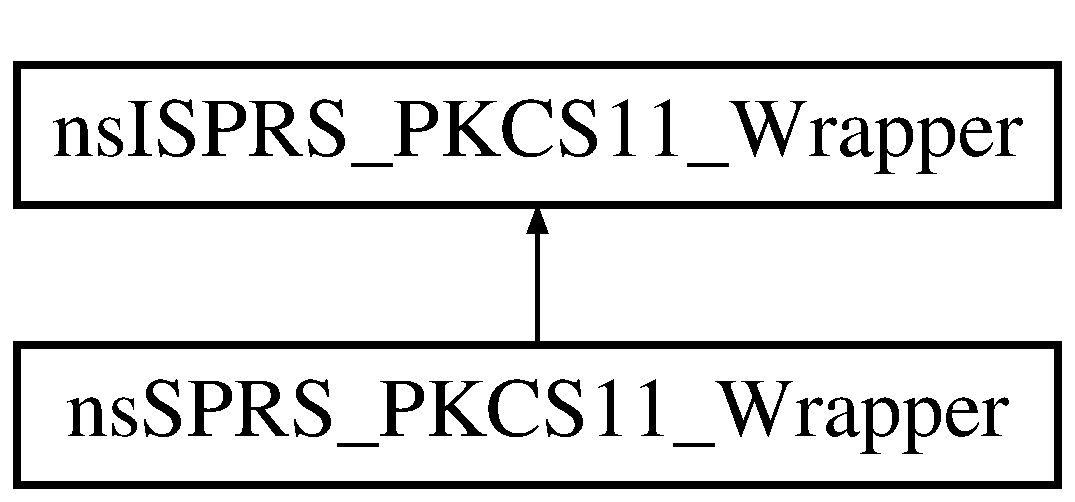
\includegraphics[height=2cm]{classnsISPRS__PKCS11__Wrapper}
\end{center}
\end{figure}
\subsection*{Public Member Functions}
\begin{DoxyCompactItemize}
\item 
\hypertarget{classnsISPRS__PKCS11__Wrapper_a8b61744812237ba63b1d6078a7140850}{
NS\_\-IMETHOD {\bfseries SPRS\_\-getLastError} (PRInt32 $\ast$\_\-retval)=0}
\label{classnsISPRS__PKCS11__Wrapper_a8b61744812237ba63b1d6078a7140850}

\item 
\hypertarget{classnsISPRS__PKCS11__Wrapper_add3cdf2b5b2bb0fe00e0f0b881185043}{
NS\_\-IMETHOD {\bfseries SPRS\_\-initCrypto} (PRBool $\ast$\_\-retval)=0}
\label{classnsISPRS__PKCS11__Wrapper_add3cdf2b5b2bb0fe00e0f0b881185043}

\item 
\hypertarget{classnsISPRS__PKCS11__Wrapper_a7f251f3a01110110ba3ed2efefc4f09f}{
NS\_\-IMETHOD {\bfseries SPRS\_\-finalizeCrypto} (void)=0}
\label{classnsISPRS__PKCS11__Wrapper_a7f251f3a01110110ba3ed2efefc4f09f}

\item 
\hypertarget{classnsISPRS__PKCS11__Wrapper_a25acd085528efa457da74b5d7a5d7939}{
NS\_\-IMETHOD {\bfseries SPRS\_\-enumerateCards} (PRUint32 $\ast$count, char $\ast$$\ast$$\ast$cards)=0}
\label{classnsISPRS__PKCS11__Wrapper_a25acd085528efa457da74b5d7a5d7939}

\item 
\hypertarget{classnsISPRS__PKCS11__Wrapper_a48e756de78fe5eb3542704505d62a543}{
NS\_\-IMETHOD {\bfseries GetArray} (PRUint32 $\ast$count, PRInt32 $\ast$$\ast$retv)=0}
\label{classnsISPRS__PKCS11__Wrapper_a48e756de78fe5eb3542704505d62a543}

\item 
\hypertarget{classnsISPRS__PKCS11__Wrapper_ac9a82527bf2c835839532302b64d3ada}{
NS\_\-IMETHOD {\bfseries SPRS\_\-selectCard} (PRInt32 card, const nsAString \&pin, PRBool $\ast$\_\-retval)=0}
\label{classnsISPRS__PKCS11__Wrapper_ac9a82527bf2c835839532302b64d3ada}

\item 
\hypertarget{classnsISPRS__PKCS11__Wrapper_a9817e5d58cb533d81e4bcf129d05cccb}{
NS\_\-IMETHOD {\bfseries SPRS\_\-listCerts} (PRUint32 $\ast$count, char $\ast$$\ast$$\ast$certs)=0}
\label{classnsISPRS__PKCS11__Wrapper_a9817e5d58cb533d81e4bcf129d05cccb}

\item 
\hypertarget{classnsISPRS__PKCS11__Wrapper_a985c8fdb86adba1b1c5f1bf33240d43a}{
NS\_\-IMETHOD {\bfseries SPRS\_\-createCert} (const nsAString \&cert, PRBool $\ast$\_\-retval)=0}
\label{classnsISPRS__PKCS11__Wrapper_a985c8fdb86adba1b1c5f1bf33240d43a}

\item 
\hypertarget{classnsISPRS__PKCS11__Wrapper_af54922c905efcea0787d2a874d9a89a5}{
NS\_\-IMETHOD {\bfseries SPRS\_\-encryptFile} (const nsAString \&input\_\-file, const nsAString \&output\_\-file, const nsAString \&cert, PRBool $\ast$\_\-retval)=0}
\label{classnsISPRS__PKCS11__Wrapper_af54922c905efcea0787d2a874d9a89a5}

\item 
\hypertarget{classnsISPRS__PKCS11__Wrapper_a75f07f75db48863b369f7737322290af}{
NS\_\-IMETHOD {\bfseries SPRS\_\-signFile} (const nsAString \&input\_\-file, const nsAString \&output\_\-file, const nsAString \&cert, PRBool $\ast$\_\-retval)=0}
\label{classnsISPRS__PKCS11__Wrapper_a75f07f75db48863b369f7737322290af}

\item 
\hypertarget{classnsISPRS__PKCS11__Wrapper_ab427cbee7f436f59428c4623e60c0241}{
NS\_\-IMETHOD {\bfseries SPRS\_\-decrypt} (const nsAString \&input\_\-file, nsAString $\ast$$\ast$\_\-retval)=0}
\label{classnsISPRS__PKCS11__Wrapper_ab427cbee7f436f59428c4623e60c0241}

\item 
\hypertarget{classnsISPRS__PKCS11__Wrapper_ab7a5864e8c3884b39b76d87cf8bf7a29}{
NS\_\-IMETHOD {\bfseries SPRS\_\-verify} (const nsAString \&input\_\-file, nsAString $\ast$$\ast$\_\-retval)=0}
\label{classnsISPRS__PKCS11__Wrapper_ab7a5864e8c3884b39b76d87cf8bf7a29}

\item 
\hypertarget{classnsISPRS__PKCS11__Wrapper_a4014c1fdcaa95ba3655b68c68d03721c}{
NS\_\-IMETHOD {\bfseries SPRS\_\-loadFile} (const nsAString \&input\_\-file, nsAString \&output, PRBool $\ast$\_\-retval)=0}
\label{classnsISPRS__PKCS11__Wrapper_a4014c1fdcaa95ba3655b68c68d03721c}

\item 
\hypertarget{classnsISPRS__PKCS11__Wrapper_a0fb1d00e8b1e8c0d72a393c3dfcadbc9}{
NS\_\-IMETHOD {\bfseries SPRS\_\-getTokenCount} (PRInt32 $\ast$\_\-retval)=0}
\label{classnsISPRS__PKCS11__Wrapper_a0fb1d00e8b1e8c0d72a393c3dfcadbc9}

\item 
\hypertarget{classnsISPRS__PKCS11__Wrapper_aa1a33b3f4065b99d44dc5d8607ad0487}{
long {\bfseries SPRS\_\-getLastError} ()}
\label{classnsISPRS__PKCS11__Wrapper_aa1a33b3f4065b99d44dc5d8607ad0487}

\item 
\hypertarget{classnsISPRS__PKCS11__Wrapper_a0ae334160bc947c3ba068ad2bc12e683}{
boolean {\bfseries SPRS\_\-initCrypto} ()}
\label{classnsISPRS__PKCS11__Wrapper_a0ae334160bc947c3ba068ad2bc12e683}

\item 
\hypertarget{classnsISPRS__PKCS11__Wrapper_a64a6e7824caf4c175e8f1b4fb18c7f4e}{
void {\bfseries SPRS\_\-finalizeCrypto} ()}
\label{classnsISPRS__PKCS11__Wrapper_a64a6e7824caf4c175e8f1b4fb18c7f4e}

\item 
\hypertarget{classnsISPRS__PKCS11__Wrapper_aa9be6c1fd0973916152ad82fd60e186a}{
void {\bfseries SPRS\_\-enumerateCards} (out PRUint32 count,\mbox{[}retval, array, size\_\-is(count)\mbox{]} out string cards)}
\label{classnsISPRS__PKCS11__Wrapper_aa9be6c1fd0973916152ad82fd60e186a}

\item 
\hypertarget{classnsISPRS__PKCS11__Wrapper_a127c335a5ec8ba9ad64218beda932e49}{
void {\bfseries getArray} (out unsigned long count,\mbox{[}array, size\_\-is(count), retval\mbox{]} out long retv)}
\label{classnsISPRS__PKCS11__Wrapper_a127c335a5ec8ba9ad64218beda932e49}

\item 
\hypertarget{classnsISPRS__PKCS11__Wrapper_ae1d9a88278e5fc06fd68c36db061e814}{
boolean {\bfseries SPRS\_\-selectCard} (in long card, in AString pin)}
\label{classnsISPRS__PKCS11__Wrapper_ae1d9a88278e5fc06fd68c36db061e814}

\item 
\hypertarget{classnsISPRS__PKCS11__Wrapper_aaad4ef266e0a525e99763d32497e968e}{
void {\bfseries SPRS\_\-listCerts} (out PRUint32 count,\mbox{[}retval, array, size\_\-is(count)\mbox{]} out string certs)}
\label{classnsISPRS__PKCS11__Wrapper_aaad4ef266e0a525e99763d32497e968e}

\item 
\hypertarget{classnsISPRS__PKCS11__Wrapper_ae276d3e673f616d997e2f01efb61666e}{
boolean {\bfseries SPRS\_\-createCert} (in AString cert)}
\label{classnsISPRS__PKCS11__Wrapper_ae276d3e673f616d997e2f01efb61666e}

\item 
\hypertarget{classnsISPRS__PKCS11__Wrapper_aef0c4b224729d300b574673e4d5ed9b9}{
boolean {\bfseries SPRS\_\-encryptFile} (in AString input\_\-file, in AString output\_\-file, in AString cert)}
\label{classnsISPRS__PKCS11__Wrapper_aef0c4b224729d300b574673e4d5ed9b9}

\item 
\hypertarget{classnsISPRS__PKCS11__Wrapper_a12fd84a1bfdadca5898a97674abcc7d2}{
boolean {\bfseries SPRS\_\-signFile} (in AString input\_\-file, in AString output\_\-file, in AString cert)}
\label{classnsISPRS__PKCS11__Wrapper_a12fd84a1bfdadca5898a97674abcc7d2}

\item 
\hypertarget{classnsISPRS__PKCS11__Wrapper_a29ba55c7ae20fe78275247a5122817cc}{
nsAString {\bfseries SPRS\_\-decrypt} (in AString input\_\-file)}
\label{classnsISPRS__PKCS11__Wrapper_a29ba55c7ae20fe78275247a5122817cc}

\item 
\hypertarget{classnsISPRS__PKCS11__Wrapper_a689e52a981017658e697a91de211cac4}{
nsAString {\bfseries SPRS\_\-verify} (in AString input\_\-file)}
\label{classnsISPRS__PKCS11__Wrapper_a689e52a981017658e697a91de211cac4}

\item 
\hypertarget{classnsISPRS__PKCS11__Wrapper_ad4590f99278e01515bafe280b1d80faf}{
boolean {\bfseries SPRS\_\-loadFile} (in AString input\_\-file, out AString output)}
\label{classnsISPRS__PKCS11__Wrapper_ad4590f99278e01515bafe280b1d80faf}

\item 
\hypertarget{classnsISPRS__PKCS11__Wrapper_aeb44d733b48bfd31ca69b803bb120387}{
long {\bfseries SPRS\_\-getTokenCount} ()}
\label{classnsISPRS__PKCS11__Wrapper_aeb44d733b48bfd31ca69b803bb120387}

\end{DoxyCompactItemize}


The documentation for this interface was generated from the following files:\begin{DoxyCompactItemize}
\item 
xpcom\_\-wrapper\_\-interface.h\item 
xpcom\_\-wrapper\_\-interface.idl\end{DoxyCompactItemize}

\hypertarget{classnsPSRS__PKCS11__Wrapper}{
\section{nsPSRS\_\-PKCS11\_\-Wrapper Class Reference}
\label{classnsPSRS__PKCS11__Wrapper}\index{nsPSRS\_\-PKCS11\_\-Wrapper@{nsPSRS\_\-PKCS11\_\-Wrapper}}
}


XPCOM component exposing CryptoWrapper to JavaScript.  


\subsection{Detailed Description}
XPCOM component exposing CryptoWrapper to JavaScript. 

The documentation for this class was generated from the following file:\begin{DoxyCompactItemize}
\item 
xpcom\_\-wrapper\_\-interface-\/impl.cpp\end{DoxyCompactItemize}

\hypertarget{classnsSPRS__PKCS11__Wrapper}{
\section{nsSPRS\_\-PKCS11\_\-Wrapper Class Reference}
\label{classnsSPRS__PKCS11__Wrapper}\index{nsSPRS\_\-PKCS11\_\-Wrapper@{nsSPRS\_\-PKCS11\_\-Wrapper}}
}
Inheritance diagram for nsSPRS\_\-PKCS11\_\-Wrapper::\begin{figure}[H]
\begin{center}
\leavevmode
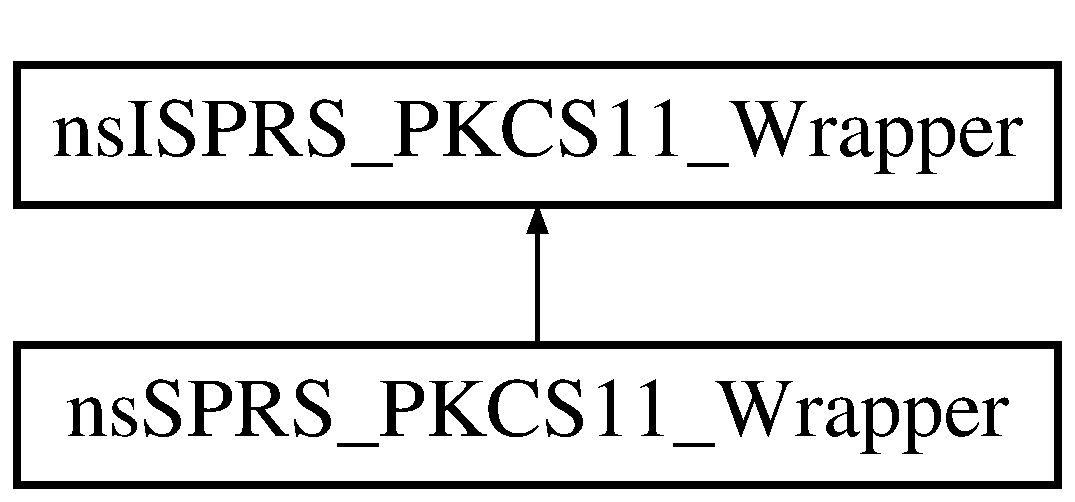
\includegraphics[height=2cm]{classnsSPRS__PKCS11__Wrapper}
\end{center}
\end{figure}
\subsection*{Public Member Functions}
\begin{DoxyCompactItemize}
\item 
NS\_\-DECL\_\-ISUPPORTS NS\_\-DECL\_\-NSISPRS\_\-PKCS11\_\-WRAPPER \hyperlink{classnsSPRS__PKCS11__Wrapper_aae53c562eb02e180de0efd9e38a8a13a}{nsSPRS\_\-PKCS11\_\-Wrapper} ()
\begin{DoxyCompactList}\small\item\em Constructor for nsSPRS\_\-PKCS11\_\-Warpper. \item\end{DoxyCompactList}\item 
\hyperlink{classnsSPRS__PKCS11__Wrapper_ae47d3a38404472caa713ff194f085cf5}{$\sim$nsSPRS\_\-PKCS11\_\-Wrapper} ()
\begin{DoxyCompactList}\small\item\em Destructor for nsSPRS\_\-PKCS11\_\-Warpper. \item\end{DoxyCompactList}\item 
NS\_\-IMETHODIMP \hyperlink{classnsSPRS__PKCS11__Wrapper_a5f2388ba9ac1bfc39f78b872ede8b877}{SPRS\_\-getLastError} (PRInt32 $\ast$\_\-retVal)
\begin{DoxyCompactList}\small\item\em calls CryptoWrapper.getLastError() \item\end{DoxyCompactList}\item 
NS\_\-IMETHODIMP \hyperlink{classnsSPRS__PKCS11__Wrapper_a474e38625c00c8a61bb890e2db670682}{SPRS\_\-initCrypto} (PRBool $\ast$\_\-retval)
\begin{DoxyCompactList}\small\item\em calls CryptoWrapper.initCrypto() \item\end{DoxyCompactList}\item 
NS\_\-IMETHODIMP \hyperlink{classnsSPRS__PKCS11__Wrapper_ab27291133f224017cdaadcceaa0b52c8}{SPRS\_\-finalizeCrypto} ()
\begin{DoxyCompactList}\small\item\em calls CryptoWrapper.finalizeCrypto() \item\end{DoxyCompactList}\item 
NS\_\-IMETHODIMP \hyperlink{classnsSPRS__PKCS11__Wrapper_aacfd858ce01bfef5569c28b8f91b4f90}{SPRS\_\-enumerateCards} (PRUint32 $\ast$count, char $\ast$$\ast$$\ast$cards)
\begin{DoxyCompactList}\small\item\em calls CryptoWrapper.enumerateCards() \item\end{DoxyCompactList}\item 
NS\_\-IMETHODIMP \hyperlink{classnsSPRS__PKCS11__Wrapper_af5ef8c8041adef789e6e6d3d38237a2b}{SPRS\_\-selectCard} (PRInt32 card, const nsAString \&pin, PRBool $\ast$\_\-retval)
\begin{DoxyCompactList}\small\item\em calls CryptoWrapper.selectCard() \item\end{DoxyCompactList}\item 
NS\_\-IMETHODIMP \hyperlink{classnsSPRS__PKCS11__Wrapper_a41711bc3e37111e22ef0bf7eaacdbc13}{SPRS\_\-listCerts} (PRUint32 $\ast$count, char $\ast$$\ast$$\ast$certs)
\begin{DoxyCompactList}\small\item\em calls CryptoWrapper.listCerts() \item\end{DoxyCompactList}\item 
NS\_\-IMETHODIMP \hyperlink{classnsSPRS__PKCS11__Wrapper_a77930438f26ec1bafd8ab07e8346af26}{SPRS\_\-encryptFile} (const nsAString \&input, const nsAString \&output, const nsAString \&cert, PRBool $\ast$\_\-retval)
\item 
NS\_\-IMETHODIMP \hyperlink{classnsSPRS__PKCS11__Wrapper_a31b12e2b457256fe858eff70590e6c83}{SPRS\_\-signFile} (const nsAString \&input\_\-file, const nsAString \&output\_\-file, const nsAString \&cert, PRBool $\ast$\_\-retval)
\item 
NS\_\-IMETHODIMP \hyperlink{classnsSPRS__PKCS11__Wrapper_a9c7932c785ee05f74583e994405183ca}{SPRS\_\-loadFile} (const nsAString \&input\_\-file, nsAString \&output, PRBool $\ast$\_\-retval)
\item 
NS\_\-IMETHODIMP \hyperlink{classnsSPRS__PKCS11__Wrapper_a91869f39a842b967711d242ce95f9637}{SPRS\_\-getTokenCount} (PRInt32 $\ast$\_\-retval)
\item 
NS\_\-IMETHODIMP \hyperlink{classnsSPRS__PKCS11__Wrapper_a592ec3f3125c461a48a66c4c88c9b118}{SPRS\_\-verify} (const nsAString \&input\_\-file, nsAString $\ast$$\ast$\_\-retval)
\begin{DoxyCompactList}\small\item\em not implemented \item\end{DoxyCompactList}\item 
NS\_\-IMETHODIMP \hyperlink{classnsSPRS__PKCS11__Wrapper_ac5b15eb2d80b960cb4f3d23e2b9b7915}{SPRS\_\-createCert} (const nsAString \&cert, PRBool $\ast$\_\-retval)
\begin{DoxyCompactList}\small\item\em not implemented \item\end{DoxyCompactList}\item 
NS\_\-IMETHODIMP \hyperlink{classnsSPRS__PKCS11__Wrapper_a167706db1c7f17e6414ec0514c45734b}{SPRS\_\-decrypt} (const nsAString \&input\_\-file, nsAString $\ast$$\ast$\_\-retval)
\begin{DoxyCompactList}\small\item\em not implemented \item\end{DoxyCompactList}\item 
NS\_\-IMETHODIMP \hyperlink{classnsSPRS__PKCS11__Wrapper_ab6151d1fd68a16d5a502ca467cb4d990}{GetArray} (PRUint32 $\ast$count, PRInt32 $\ast$$\ast$retv)
\begin{DoxyCompactList}\small\item\em Deemonstrates XPIDL array support is in fact working with SDK. \item\end{DoxyCompactList}\end{DoxyCompactItemize}
\subsection*{Protected Member Functions}
\begin{DoxyCompactItemize}
\item 
\hypertarget{classnsSPRS__PKCS11__Wrapper_a9fb490e90a235df6b273c06ba284076e}{
void {\bfseries setError} (int error)}
\label{classnsSPRS__PKCS11__Wrapper_a9fb490e90a235df6b273c06ba284076e}

\item 
\hypertarget{classnsSPRS__PKCS11__Wrapper_a603124bb2ec2f4b6abac9c077664cda7}{
bool {\bfseries initCrypto} ()}
\label{classnsSPRS__PKCS11__Wrapper_a603124bb2ec2f4b6abac9c077664cda7}

\item 
\hypertarget{classnsSPRS__PKCS11__Wrapper_aa11b58c73c6846a2f15365880703150a}{
void {\bfseries finalizeCrypto} ()}
\label{classnsSPRS__PKCS11__Wrapper_aa11b58c73c6846a2f15365880703150a}

\item 
\hypertarget{classnsSPRS__PKCS11__Wrapper_a409dd546aad42560ed8e537dc2d61abc}{
int {\bfseries getLastError} (void)}
\label{classnsSPRS__PKCS11__Wrapper_a409dd546aad42560ed8e537dc2d61abc}

\item 
\hypertarget{classnsSPRS__PKCS11__Wrapper_ae95c96664a1d6cd17a9ed5869448be0e}{
int {\bfseries getTokenCount} ()}
\label{classnsSPRS__PKCS11__Wrapper_ae95c96664a1d6cd17a9ed5869448be0e}

\item 
\hypertarget{classnsSPRS__PKCS11__Wrapper_aca888cd1ea10ac257332bd089db5888a}{
bool {\bfseries selectCard} (long slotID, const nsAString \&pin)}
\label{classnsSPRS__PKCS11__Wrapper_aca888cd1ea10ac257332bd089db5888a}

\item 
\hypertarget{classnsSPRS__PKCS11__Wrapper_aacf5801892adb8eb441e6a5c3900b906}{
string $\ast$ {\bfseries enumerateCards} (void)}
\label{classnsSPRS__PKCS11__Wrapper_aacf5801892adb8eb441e6a5c3900b906}

\end{DoxyCompactItemize}


\subsection{Constructor \& Destructor Documentation}
\hypertarget{classnsSPRS__PKCS11__Wrapper_aae53c562eb02e180de0efd9e38a8a13a}{
\index{nsSPRS\_\-PKCS11\_\-Wrapper@{nsSPRS\_\-PKCS11\_\-Wrapper}!nsSPRS\_\-PKCS11\_\-Wrapper@{nsSPRS\_\-PKCS11\_\-Wrapper}}
\index{nsSPRS\_\-PKCS11\_\-Wrapper@{nsSPRS\_\-PKCS11\_\-Wrapper}!nsSPRS_PKCS11_Wrapper@{nsSPRS\_\-PKCS11\_\-Wrapper}}
\subsubsection[{nsSPRS\_\-PKCS11\_\-Wrapper}]{\setlength{\rightskip}{0pt plus 5cm}nsSPRS\_\-PKCS11\_\-Wrapper::nsSPRS\_\-PKCS11\_\-Wrapper ()}}
\label{classnsSPRS__PKCS11__Wrapper_aae53c562eb02e180de0efd9e38a8a13a}


Constructor for nsSPRS\_\-PKCS11\_\-Warpper. \begin{DoxyRemark}{Remarks}
does nothing interesting 
\end{DoxyRemark}
\hypertarget{classnsSPRS__PKCS11__Wrapper_ae47d3a38404472caa713ff194f085cf5}{
\index{nsSPRS\_\-PKCS11\_\-Wrapper@{nsSPRS\_\-PKCS11\_\-Wrapper}!$\sim$nsSPRS\_\-PKCS11\_\-Wrapper@{$\sim$nsSPRS\_\-PKCS11\_\-Wrapper}}
\index{$\sim$nsSPRS\_\-PKCS11\_\-Wrapper@{$\sim$nsSPRS\_\-PKCS11\_\-Wrapper}!nsSPRS_PKCS11_Wrapper@{nsSPRS\_\-PKCS11\_\-Wrapper}}
\subsubsection[{$\sim$nsSPRS\_\-PKCS11\_\-Wrapper}]{\setlength{\rightskip}{0pt plus 5cm}nsSPRS\_\-PKCS11\_\-Wrapper::$\sim$nsSPRS\_\-PKCS11\_\-Wrapper ()}}
\label{classnsSPRS__PKCS11__Wrapper_ae47d3a38404472caa713ff194f085cf5}


Destructor for nsSPRS\_\-PKCS11\_\-Warpper. \begin{DoxyRemark}{Remarks}
does nothing interesting 
\end{DoxyRemark}


\subsection{Member Function Documentation}
\hypertarget{classnsSPRS__PKCS11__Wrapper_ab6151d1fd68a16d5a502ca467cb4d990}{
\index{nsSPRS\_\-PKCS11\_\-Wrapper@{nsSPRS\_\-PKCS11\_\-Wrapper}!GetArray@{GetArray}}
\index{GetArray@{GetArray}!nsSPRS_PKCS11_Wrapper@{nsSPRS\_\-PKCS11\_\-Wrapper}}
\subsubsection[{GetArray}]{\setlength{\rightskip}{0pt plus 5cm}NS\_\-IMETHODIMP nsSPRS\_\-PKCS11\_\-Wrapper::GetArray (PRUint32 $\ast$ {\em count}, \/  PRInt32 $\ast$$\ast$ {\em retv})\hspace{0.3cm}{\ttfamily  \mbox{[}virtual\mbox{]}}}}
\label{classnsSPRS__PKCS11__Wrapper_ab6151d1fd68a16d5a502ca467cb4d990}


Deemonstrates XPIDL array support is in fact working with SDK. This is not part of the wrapper API, it's just a sanity check. Returns an array with 10 elements. JavaScript signature: void getArray (out unsigned long count, \mbox{[}array, size\_\-is (count), retval\mbox{]} out long retv);

This is called from JavaScript like this: var count = \{\}; var arr = obj.getArray(count); alert(\char`\"{}Count.value: \char`\"{} + count.value); alert(\char`\"{}Cards: \char`\"{} + arr);


\begin{DoxyRetVals}{Return values}
\item[{\em NS\_\-IMETHODIMP}]NS\_\-OK \end{DoxyRetVals}
\begin{DoxyRemark}{Remarks}
This is not part of the wrapper API, it's just a sanity check. 
\end{DoxyRemark}


Implements \hyperlink{classnsISPRS__PKCS11__Wrapper}{nsISPRS\_\-PKCS11\_\-Wrapper}.\hypertarget{classnsSPRS__PKCS11__Wrapper_ac5b15eb2d80b960cb4f3d23e2b9b7915}{
\index{nsSPRS\_\-PKCS11\_\-Wrapper@{nsSPRS\_\-PKCS11\_\-Wrapper}!SPRS\_\-createCert@{SPRS\_\-createCert}}
\index{SPRS\_\-createCert@{SPRS\_\-createCert}!nsSPRS_PKCS11_Wrapper@{nsSPRS\_\-PKCS11\_\-Wrapper}}
\subsubsection[{SPRS\_\-createCert}]{\setlength{\rightskip}{0pt plus 5cm}NS\_\-IMETHODIMP nsSPRS\_\-PKCS11\_\-Wrapper::SPRS\_\-createCert (const nsAString \& {\em cert}, \/  PRBool $\ast$ {\em \_\-retval})\hspace{0.3cm}{\ttfamily  \mbox{[}virtual\mbox{]}}}}
\label{classnsSPRS__PKCS11__Wrapper_ac5b15eb2d80b960cb4f3d23e2b9b7915}


not implemented 
\begin{DoxyRetVals}{Return values}
\item[{\em NS\_\-IMETHODIMP}]NS\_\-ERROR\_\-NOT\_\-IMPLEMENTED \end{DoxyRetVals}
\begin{DoxyRemark}{Remarks}
Calling this will result in a not implemented exception! 
\end{DoxyRemark}


Implements \hyperlink{classnsISPRS__PKCS11__Wrapper}{nsISPRS\_\-PKCS11\_\-Wrapper}.\hypertarget{classnsSPRS__PKCS11__Wrapper_a167706db1c7f17e6414ec0514c45734b}{
\index{nsSPRS\_\-PKCS11\_\-Wrapper@{nsSPRS\_\-PKCS11\_\-Wrapper}!SPRS\_\-decrypt@{SPRS\_\-decrypt}}
\index{SPRS\_\-decrypt@{SPRS\_\-decrypt}!nsSPRS_PKCS11_Wrapper@{nsSPRS\_\-PKCS11\_\-Wrapper}}
\subsubsection[{SPRS\_\-decrypt}]{\setlength{\rightskip}{0pt plus 5cm}NS\_\-IMETHODIMP nsSPRS\_\-PKCS11\_\-Wrapper::SPRS\_\-decrypt (const nsAString \& {\em input\_\-file}, \/  nsAString $\ast$$\ast$ {\em \_\-retval})\hspace{0.3cm}{\ttfamily  \mbox{[}virtual\mbox{]}}}}
\label{classnsSPRS__PKCS11__Wrapper_a167706db1c7f17e6414ec0514c45734b}


not implemented 
\begin{DoxyRetVals}{Return values}
\item[{\em NS\_\-IMETHODIMP}]NS\_\-ERROR\_\-NOT\_\-IMPLEMENTED \end{DoxyRetVals}
\begin{DoxyRemark}{Remarks}
Calling this will result in a not implemented exception! 
\end{DoxyRemark}


Implements \hyperlink{classnsISPRS__PKCS11__Wrapper}{nsISPRS\_\-PKCS11\_\-Wrapper}.\hypertarget{classnsSPRS__PKCS11__Wrapper_a77930438f26ec1bafd8ab07e8346af26}{
\index{nsSPRS\_\-PKCS11\_\-Wrapper@{nsSPRS\_\-PKCS11\_\-Wrapper}!SPRS\_\-encryptFile@{SPRS\_\-encryptFile}}
\index{SPRS\_\-encryptFile@{SPRS\_\-encryptFile}!nsSPRS_PKCS11_Wrapper@{nsSPRS\_\-PKCS11\_\-Wrapper}}
\subsubsection[{SPRS\_\-encryptFile}]{\setlength{\rightskip}{0pt plus 5cm}NS\_\-IMETHODIMP nsSPRS\_\-PKCS11\_\-Wrapper::SPRS\_\-encryptFile (const nsAString \& {\em input}, \/  const nsAString \& {\em output}, \/  const nsAString \& {\em cert}, \/  PRBool $\ast$ {\em \_\-retval})\hspace{0.3cm}{\ttfamily  \mbox{[}virtual\mbox{]}}}}
\label{classnsSPRS__PKCS11__Wrapper_a77930438f26ec1bafd8ab07e8346af26}
JavaScript signature: boolean signFile(in nsAString input\_\-file, in nsAString output\_\-file, in nsAString cert); 
\begin{DoxyParams}{Parameters}
\item[\mbox{$\leftarrow$} {\em input}]name of input file \item[\mbox{$\leftarrow$} {\em output}]name of output file \item[\mbox{$\leftarrow$} {\em cert}]name of certificate to use for encryption \item[\mbox{$\rightarrow$} {\em \_\-retval}]success/failure of CryptoWrapper.encryptFile() \end{DoxyParams}

\begin{DoxyRetVals}{Return values}
\item[{\em NS\_\-IMETHODIMP}]NS\_\-OK \end{DoxyRetVals}
\begin{DoxyRemark}{Remarks}
calls CryptoWrapper.encryptFile() 
\end{DoxyRemark}


Implements \hyperlink{classnsISPRS__PKCS11__Wrapper}{nsISPRS\_\-PKCS11\_\-Wrapper}.\hypertarget{classnsSPRS__PKCS11__Wrapper_aacfd858ce01bfef5569c28b8f91b4f90}{
\index{nsSPRS\_\-PKCS11\_\-Wrapper@{nsSPRS\_\-PKCS11\_\-Wrapper}!SPRS\_\-enumerateCards@{SPRS\_\-enumerateCards}}
\index{SPRS\_\-enumerateCards@{SPRS\_\-enumerateCards}!nsSPRS_PKCS11_Wrapper@{nsSPRS\_\-PKCS11\_\-Wrapper}}
\subsubsection[{SPRS\_\-enumerateCards}]{\setlength{\rightskip}{0pt plus 5cm}NS\_\-IMETHODIMP nsSPRS\_\-PKCS11\_\-Wrapper::SPRS\_\-enumerateCards (PRUint32 $\ast$ {\em count}, \/  char $\ast$$\ast$$\ast$ {\em cards})\hspace{0.3cm}{\ttfamily  \mbox{[}virtual\mbox{]}}}}
\label{classnsSPRS__PKCS11__Wrapper_aacfd858ce01bfef5569c28b8f91b4f90}


calls CryptoWrapper.enumerateCards() JavaScript signature: nsIArray \hyperlink{classnsSPRS__PKCS11__Wrapper_aacfd858ce01bfef5569c28b8f91b4f90}{SPRS\_\-enumerateCards()};


\begin{DoxyParams}{Parameters}
\item[\mbox{$\rightarrow$} {\em count}]number of cards detected \item[\mbox{$\rightarrow$} {\em cards}]array of strings of card names \end{DoxyParams}

\begin{DoxyRetVals}{Return values}
\item[{\em NS\_\-IMETHODIMP}]NS\_\-OK or NS\_\-ERROR\_\-OUT\_\-OF\_\-MEMORY \end{DoxyRetVals}
\begin{DoxyRemark}{Remarks}
calls CryptoWrapper.enumerateCards() 
\end{DoxyRemark}


Implements \hyperlink{classnsISPRS__PKCS11__Wrapper}{nsISPRS\_\-PKCS11\_\-Wrapper}.\hypertarget{classnsSPRS__PKCS11__Wrapper_ab27291133f224017cdaadcceaa0b52c8}{
\index{nsSPRS\_\-PKCS11\_\-Wrapper@{nsSPRS\_\-PKCS11\_\-Wrapper}!SPRS\_\-finalizeCrypto@{SPRS\_\-finalizeCrypto}}
\index{SPRS\_\-finalizeCrypto@{SPRS\_\-finalizeCrypto}!nsSPRS_PKCS11_Wrapper@{nsSPRS\_\-PKCS11\_\-Wrapper}}
\subsubsection[{SPRS\_\-finalizeCrypto}]{\setlength{\rightskip}{0pt plus 5cm}NS\_\-IMETHODIMP nsSPRS\_\-PKCS11\_\-Wrapper::SPRS\_\-finalizeCrypto (void)\hspace{0.3cm}{\ttfamily  \mbox{[}virtual\mbox{]}}}}
\label{classnsSPRS__PKCS11__Wrapper_ab27291133f224017cdaadcceaa0b52c8}


calls CryptoWrapper.finalizeCrypto() There is no indication of success/failure.

JavaScript signature: void \hyperlink{classnsSPRS__PKCS11__Wrapper_ab27291133f224017cdaadcceaa0b52c8}{SPRS\_\-finalizeCrypto()}; 
\begin{DoxyRetVals}{Return values}
\item[{\em NS\_\-IMETHODIMP}]NS\_\-OK \end{DoxyRetVals}
\begin{DoxyRemark}{Remarks}
calls CryptoWrapper.finalizeCrypto() 
\end{DoxyRemark}


Implements \hyperlink{classnsISPRS__PKCS11__Wrapper}{nsISPRS\_\-PKCS11\_\-Wrapper}.\hypertarget{classnsSPRS__PKCS11__Wrapper_a5f2388ba9ac1bfc39f78b872ede8b877}{
\index{nsSPRS\_\-PKCS11\_\-Wrapper@{nsSPRS\_\-PKCS11\_\-Wrapper}!SPRS\_\-getLastError@{SPRS\_\-getLastError}}
\index{SPRS\_\-getLastError@{SPRS\_\-getLastError}!nsSPRS_PKCS11_Wrapper@{nsSPRS\_\-PKCS11\_\-Wrapper}}
\subsubsection[{SPRS\_\-getLastError}]{\setlength{\rightskip}{0pt plus 5cm}NS\_\-IMETHODIMP nsSPRS\_\-PKCS11\_\-Wrapper::SPRS\_\-getLastError (PRInt32 $\ast$ {\em \_\-retval})\hspace{0.3cm}{\ttfamily  \mbox{[}virtual\mbox{]}}}}
\label{classnsSPRS__PKCS11__Wrapper_a5f2388ba9ac1bfc39f78b872ede8b877}


calls CryptoWrapper.getLastError() 
\begin{DoxyParams}{Parameters}
\item[\mbox{$\rightarrow$} {\em \_\-retval}]error code \end{DoxyParams}

\begin{DoxyRetVals}{Return values}
\item[{\em NS\_\-IMETHODIMP}]NS\_\-OK \end{DoxyRetVals}
\begin{DoxyRemark}{Remarks}
JavaScript signature: long SPRS\_\-getLastError(); 
\end{DoxyRemark}


Implements \hyperlink{classnsISPRS__PKCS11__Wrapper}{nsISPRS\_\-PKCS11\_\-Wrapper}.\hypertarget{classnsSPRS__PKCS11__Wrapper_a91869f39a842b967711d242ce95f9637}{
\index{nsSPRS\_\-PKCS11\_\-Wrapper@{nsSPRS\_\-PKCS11\_\-Wrapper}!SPRS\_\-getTokenCount@{SPRS\_\-getTokenCount}}
\index{SPRS\_\-getTokenCount@{SPRS\_\-getTokenCount}!nsSPRS_PKCS11_Wrapper@{nsSPRS\_\-PKCS11\_\-Wrapper}}
\subsubsection[{SPRS\_\-getTokenCount}]{\setlength{\rightskip}{0pt plus 5cm}NS\_\-IMETHODIMP nsSPRS\_\-PKCS11\_\-Wrapper::SPRS\_\-getTokenCount (PRInt32 $\ast$ {\em \_\-retval})\hspace{0.3cm}{\ttfamily  \mbox{[}virtual\mbox{]}}}}
\label{classnsSPRS__PKCS11__Wrapper_a91869f39a842b967711d242ce95f9637}
JavaScript signature: long SPRS\_\-getTokenCount(); 
\begin{DoxyParams}{Parameters}
\item[{\em PRInt32}]$\ast$\_\-retval number of cards/tokens detected \end{DoxyParams}

\begin{DoxyRetVals}{Return values}
\item[{\em NS\_\-IMETHODIMP}]NS\_\-OK \end{DoxyRetVals}
\begin{DoxyRemark}{Remarks}
calls CryptoWrapper.getTokenCount() 
\end{DoxyRemark}


Implements \hyperlink{classnsISPRS__PKCS11__Wrapper}{nsISPRS\_\-PKCS11\_\-Wrapper}.\hypertarget{classnsSPRS__PKCS11__Wrapper_a474e38625c00c8a61bb890e2db670682}{
\index{nsSPRS\_\-PKCS11\_\-Wrapper@{nsSPRS\_\-PKCS11\_\-Wrapper}!SPRS\_\-initCrypto@{SPRS\_\-initCrypto}}
\index{SPRS\_\-initCrypto@{SPRS\_\-initCrypto}!nsSPRS_PKCS11_Wrapper@{nsSPRS\_\-PKCS11\_\-Wrapper}}
\subsubsection[{SPRS\_\-initCrypto}]{\setlength{\rightskip}{0pt plus 5cm}NS\_\-IMETHODIMP nsSPRS\_\-PKCS11\_\-Wrapper::SPRS\_\-initCrypto (PRBool $\ast$ {\em \_\-retval})\hspace{0.3cm}{\ttfamily  \mbox{[}virtual\mbox{]}}}}
\label{classnsSPRS__PKCS11__Wrapper_a474e38625c00c8a61bb890e2db670682}


calls CryptoWrapper.initCrypto() 
\begin{DoxyParams}{Parameters}
\item[\mbox{$\rightarrow$} {\em \_\-retval}]success/failure of CryptoWrapper.initCrypto() \end{DoxyParams}

\begin{DoxyRetVals}{Return values}
\item[{\em NS\_\-IMETHODIMP}]NS\_\-OK \end{DoxyRetVals}
\begin{DoxyRemark}{Remarks}
JavaScript signature: boolean SPRS\_\-initCrypto(); 
\end{DoxyRemark}


Implements \hyperlink{classnsISPRS__PKCS11__Wrapper}{nsISPRS\_\-PKCS11\_\-Wrapper}.\hypertarget{classnsSPRS__PKCS11__Wrapper_a41711bc3e37111e22ef0bf7eaacdbc13}{
\index{nsSPRS\_\-PKCS11\_\-Wrapper@{nsSPRS\_\-PKCS11\_\-Wrapper}!SPRS\_\-listCerts@{SPRS\_\-listCerts}}
\index{SPRS\_\-listCerts@{SPRS\_\-listCerts}!nsSPRS_PKCS11_Wrapper@{nsSPRS\_\-PKCS11\_\-Wrapper}}
\subsubsection[{SPRS\_\-listCerts}]{\setlength{\rightskip}{0pt plus 5cm}NS\_\-IMETHODIMP nsSPRS\_\-PKCS11\_\-Wrapper::SPRS\_\-listCerts (PRUint32 $\ast$ {\em count}, \/  char $\ast$$\ast$$\ast$ {\em certs})\hspace{0.3cm}{\ttfamily  \mbox{[}virtual\mbox{]}}}}
\label{classnsSPRS__PKCS11__Wrapper_a41711bc3e37111e22ef0bf7eaacdbc13}


calls CryptoWrapper.listCerts() JavaScript signature: void SPRS\_\-listCerts (out PRUint32 count, \mbox{[}array, size\_\-is (count), retval\mbox{]}out string certs); 
\begin{DoxyParams}{Parameters}
\item[\mbox{$\rightarrow$} {\em count}]number of certs detected \item[\mbox{$\rightarrow$} {\em certs}]array of strings of cert names \end{DoxyParams}

\begin{DoxyRetVals}{Return values}
\item[{\em NS\_\-IMETHODIMP}]NS\_\-OK or NS\_\-ERROR\_\-OUT\_\-OF\_\-MEMORY \end{DoxyRetVals}
\begin{DoxyRemark}{Remarks}
calls CryptoWrapper.listCerts() 
\end{DoxyRemark}


Implements \hyperlink{classnsISPRS__PKCS11__Wrapper}{nsISPRS\_\-PKCS11\_\-Wrapper}.\hypertarget{classnsSPRS__PKCS11__Wrapper_a9c7932c785ee05f74583e994405183ca}{
\index{nsSPRS\_\-PKCS11\_\-Wrapper@{nsSPRS\_\-PKCS11\_\-Wrapper}!SPRS\_\-loadFile@{SPRS\_\-loadFile}}
\index{SPRS\_\-loadFile@{SPRS\_\-loadFile}!nsSPRS_PKCS11_Wrapper@{nsSPRS\_\-PKCS11\_\-Wrapper}}
\subsubsection[{SPRS\_\-loadFile}]{\setlength{\rightskip}{0pt plus 5cm}NS\_\-IMETHODIMP nsSPRS\_\-PKCS11\_\-Wrapper::SPRS\_\-loadFile (const nsAString \& {\em input\_\-file}, \/  nsAString \& {\em output}, \/  PRBool $\ast$ {\em \_\-retval})\hspace{0.3cm}{\ttfamily  \mbox{[}virtual\mbox{]}}}}
\label{classnsSPRS__PKCS11__Wrapper_a9c7932c785ee05f74583e994405183ca}
JavaScript signature: boolean SPRS\_\-loadFile (in AString input\_\-file, out AString output); 
\begin{DoxyParams}{Parameters}
\item[\mbox{$\leftarrow$} {\em input\_\-file}]name of file to load \item[\mbox{$\rightarrow$} {\em output}]string containing cleartext of input file \item[\mbox{$\rightarrow$} {\em \_\-retval}]success/failure of CryptoWrapper.loadFile() \end{DoxyParams}

\begin{DoxyRetVals}{Return values}
\item[{\em NS\_\-IMETHODIMP}]NS\_\-OK \end{DoxyRetVals}
\begin{DoxyRemark}{Remarks}
calls CryptoWrapper.loadFile() 
\end{DoxyRemark}


Implements \hyperlink{classnsISPRS__PKCS11__Wrapper}{nsISPRS\_\-PKCS11\_\-Wrapper}.\hypertarget{classnsSPRS__PKCS11__Wrapper_af5ef8c8041adef789e6e6d3d38237a2b}{
\index{nsSPRS\_\-PKCS11\_\-Wrapper@{nsSPRS\_\-PKCS11\_\-Wrapper}!SPRS\_\-selectCard@{SPRS\_\-selectCard}}
\index{SPRS\_\-selectCard@{SPRS\_\-selectCard}!nsSPRS_PKCS11_Wrapper@{nsSPRS\_\-PKCS11\_\-Wrapper}}
\subsubsection[{SPRS\_\-selectCard}]{\setlength{\rightskip}{0pt plus 5cm}NS\_\-IMETHODIMP nsSPRS\_\-PKCS11\_\-Wrapper::SPRS\_\-selectCard (PRInt32 {\em card}, \/  const nsAString \& {\em pin}, \/  PRBool $\ast$ {\em \_\-retval})\hspace{0.3cm}{\ttfamily  \mbox{[}virtual\mbox{]}}}}
\label{classnsSPRS__PKCS11__Wrapper_af5ef8c8041adef789e6e6d3d38237a2b}


calls CryptoWrapper.selectCard() JavaScript signature: boolean SPRS\_\-selectCard(in nsAString card);


\begin{DoxyParams}{Parameters}
\item[\mbox{$\leftarrow$} {\em card}]zero-\/based index of card \item[\mbox{$\leftarrow$} {\em pin}]user-\/level PIN for card \item[\mbox{$\rightarrow$} {\em \_\-retval}]success/failure of CryptoWrapper.selectCard() \end{DoxyParams}

\begin{DoxyRetVals}{Return values}
\item[{\em NS\_\-IMETHODIMP}]NS\_\-OK \end{DoxyRetVals}
\begin{DoxyRemark}{Remarks}
calls CryptoWrapper.selectCard() 
\end{DoxyRemark}


Implements \hyperlink{classnsISPRS__PKCS11__Wrapper}{nsISPRS\_\-PKCS11\_\-Wrapper}.\hypertarget{classnsSPRS__PKCS11__Wrapper_a31b12e2b457256fe858eff70590e6c83}{
\index{nsSPRS\_\-PKCS11\_\-Wrapper@{nsSPRS\_\-PKCS11\_\-Wrapper}!SPRS\_\-signFile@{SPRS\_\-signFile}}
\index{SPRS\_\-signFile@{SPRS\_\-signFile}!nsSPRS_PKCS11_Wrapper@{nsSPRS\_\-PKCS11\_\-Wrapper}}
\subsubsection[{SPRS\_\-signFile}]{\setlength{\rightskip}{0pt plus 5cm}NS\_\-IMETHODIMP nsSPRS\_\-PKCS11\_\-Wrapper::SPRS\_\-signFile (const nsAString \& {\em input\_\-file}, \/  const nsAString \& {\em output\_\-file}, \/  const nsAString \& {\em cert}, \/  PRBool $\ast$ {\em \_\-retval})\hspace{0.3cm}{\ttfamily  \mbox{[}virtual\mbox{]}}}}
\label{classnsSPRS__PKCS11__Wrapper_a31b12e2b457256fe858eff70590e6c83}
JavaScript signature: boolean signFile (in nsAString input\_\-file, in nsAString output\_\-file, in nsAString cert); 
\begin{DoxyParams}{Parameters}
\item[\mbox{$\leftarrow$} {\em input\_\-file}]name of input file \item[\mbox{$\leftarrow$} {\em output\_\-file}]name of output file \item[\mbox{$\leftarrow$} {\em cert}]name of certificate to use for signing \item[\mbox{$\rightarrow$} {\em \_\-retval}]success/failure of CryptoWrapper.signFile() \end{DoxyParams}

\begin{DoxyRetVals}{Return values}
\item[{\em NS\_\-IMETHODIMP}]NS\_\-OK \end{DoxyRetVals}
\begin{DoxyRemark}{Remarks}
calls CryptoWrapper.signFile() 
\end{DoxyRemark}


Implements \hyperlink{classnsISPRS__PKCS11__Wrapper}{nsISPRS\_\-PKCS11\_\-Wrapper}.\hypertarget{classnsSPRS__PKCS11__Wrapper_a592ec3f3125c461a48a66c4c88c9b118}{
\index{nsSPRS\_\-PKCS11\_\-Wrapper@{nsSPRS\_\-PKCS11\_\-Wrapper}!SPRS\_\-verify@{SPRS\_\-verify}}
\index{SPRS\_\-verify@{SPRS\_\-verify}!nsSPRS_PKCS11_Wrapper@{nsSPRS\_\-PKCS11\_\-Wrapper}}
\subsubsection[{SPRS\_\-verify}]{\setlength{\rightskip}{0pt plus 5cm}NS\_\-IMETHODIMP nsSPRS\_\-PKCS11\_\-Wrapper::SPRS\_\-verify (const nsAString \& {\em input\_\-file}, \/  nsAString $\ast$$\ast$ {\em \_\-retval})\hspace{0.3cm}{\ttfamily  \mbox{[}virtual\mbox{]}}}}
\label{classnsSPRS__PKCS11__Wrapper_a592ec3f3125c461a48a66c4c88c9b118}


not implemented 
\begin{DoxyRetVals}{Return values}
\item[{\em NS\_\-IMETHODIMP}]NS\_\-ERROR\_\-NOT\_\-IMPLEMENTED \end{DoxyRetVals}
\begin{DoxyRemark}{Remarks}
Calling this will result in a not implemented exception! 
\end{DoxyRemark}


Implements \hyperlink{classnsISPRS__PKCS11__Wrapper}{nsISPRS\_\-PKCS11\_\-Wrapper}.

The documentation for this class was generated from the following files:\begin{DoxyCompactItemize}
\item 
xpcom\_\-wrapper\_\-interface-\/impl.h\item 
xpcom\_\-wrapper\_\-interface-\/impl.cpp\end{DoxyCompactItemize}

\printindex
\end{document}
